\subsection{\textbf{RQ2:} What factors impact the difficulty of a conflict resolution?}\label{RQ2}

\todo{talk about resolution difficulties in interviews and how survey answer options were formed}
\todo{double check card descriptions with actual cards}

\begin{table}[!]
\renewcommand{\arraystretch}{1.3}
\caption{Merge Conflict Resolution Difficulty Categories from Interviews}
\label{interview_tags_rq2}
\centering
\begin{tabularx}{0.5\textwidth}{@{}{c}@{ }{c}@{ }p{4.4cm}}
\toprule
	Category & \# Cards & \hfil Description \\
\midrule

\textit{Code Comprehensibility}	& 9 & How people understand what makes the conflict difficult. \\
\textit{Archeology} & 8 & Exploring a project's history. \\
\textit{Maintaining Behavior} & 5 & Program behavior should not change because of the conflict. \\
\textit{Complex Project Structure} & 4 & Increased difficulty because the project is more complex. \\
\textit{Knowledge Gap} & 4 & Practitioners lack the knowledge necessary to resolve a merge conflict. \\
\textit{Shifting Assumptions	} & 3 & Code-based assumptions are different between two code versions. \\
\textit{Dependency Hell} & 3 & References to external code or other parts of the system make resolution more complicated. \\
\textit{Commit Messages}	 & 3 & The impact of commit message content. \\
\textit{Territorial Contributors} &	2 & Some contributors have perceived ownership over sections of code which must be respected. \\
\textit{Legacy Code} & 1 & Old code where the original author is no longer accessible. \\

\bottomrule
\end{tabularx}
\end{table}

\subsubsection{General}

Our interviews resulted in 10 categories in this category, as shown in Table \ref{interview_tags_rq2}.

For this section in the survey, 141 participants rated how much each factor affects the difficulty of resolving merge conflicts and were given the following options:

\begin{enumerate}
	\item \textit{Not at all}
	\item \textit{A little}
	\item \textit{A moderate amount}
	\item \textit{A lot}
	\item \textit{A great deal}
\end{enumerate}
The results for this section are given in Table \ref{survey_res_diffs}, which highlights three of the factors which show stronger developer opinions:
\begin{itemize}
\item \textit{How easy it is to understand the code involved in the merge conflict}. 
\item \textit{Your expertise in the area of code with the merge conflict}
\item \textit{The amount of information you have about the conflicting code} 
\end{itemize} 

\begin{table*}[!]
\renewcommand{\arraystretch}{1.3}
\caption{Difficulties in Resolving a Merge Conflict from Survey}
\label{survey_res_diffs}
\centering
\begin{tabularx}{0.9\textwidth}{r | *5{c} | *3{c}}

\toprule
	Factor & 1 & 2 & 3 & 4 & 5 & Mean & Median & Std. Dev. \\
\midrule
	\textbf{How easy it is to understand the code involved in the merge conflict} & 0 & 14 & 25 & 65 & 37 & \textbf{3.89} & 4 & 0.91\\
	\textbf{Your expertise in the area of code with the merge conflict} & 1 & 17 & 38 & 49 & 36 & \textbf{3.72} & 4 & 1.00\\
	\textbf{The amount of information you have about the conflicting code} & 2 & 21 & 38 & 48 & 32 & \textbf{3.62} & 4 & 1.04\\
	How well tools present information in an understandable way & 4 & 24 & 47 & 32 & 34 & 3.48 & 3 & 1.12\\
	Changing assumptions within the code & 8 & 27 & 45 & 36 & 25 & 3.30 & 3 & 1.14\\
	Complexity of the project structure & 6 & 38 & 39 & 41 & 17 & 3.18 & 3 & 1.09\\
	Trustworthiness of tools & 17 & 29 & 39 & 32 & 34 & 3.12 & 3 & 1.26\\
	Informativeness of commit messages & 18 & 32 & 30 & 44 & 17 & 3.07 & 3 & 1.24\\
	Project Culture & 13 & 37 & 43 & 27 & 21 & 3.04 & 3 & 1.19\\
	Tool support for examining development history & 16 & 40 & 31 & 32 & 22 & 3.03 & 3 & 1.26\\
\bottomrule
\end{tabularx}
\end{table*}

No factor in this category had an average below 3.03, so there were no factors tested that were rated as having less than a moderate amount of affect on the difficulty of a merge conflict resolution.

\subsubsection{Commit Messages}
Based on prior work stating the value of commit messages~\cite{yamauchi2014clustering}\cite{hindle2009automatic}\cite{cortes2014automatically}\cite{hattori2008nature}, we expected commit messages to be a helpful tool in merge conflict resolution. 
P10 agrees with this, but still wishes that commit messages could be more informative:
\begin{displayquote}
	\textit{That really helps in making decisions on... two commits that have done something similar, and one commit has done some additional work... then I know that this commit has additional changes and I should look out for those when I'm resolving the merge conflict. So yeah, more information in commit messages would definitely help.}
\end{displayquote}

In contrast, P5 says that commit messages just aren't descriptive enough:
\begin{displayquote}
\textit{I wont understand from just the commit messages what the other person was trying to do... I just won't have enough information to resolve the merge.}
\end{displayquote}

P4 compared his past experience working in industry and his current work on open-source academic research software, explaining that developer messages from more experienced professionals are helpful, but gets more vague commit messages from \textit{``less experienced developers, students, post-docs, guys who are just used to not even using source control.''}

Given this mixed information about commit messages in the interviews, we further investigated developer perceptions in the survey and found that software practitioners believe that \textit{Informativeness of commit messages} has a moderate impact (mean 3.03) on the difficulty of a merge conflict resolution. making it the 8th  of the 10 factors we asked about (see Table \ref{survey_res_diffs}). One possible explanation for this discrepancy between the literature and perceptions is that commit messages provide a good source of metadata for researchers mining software repositories, but they are often too short or vague to provide helpful information about the commits involved in a conflict.
\subsubsection{Code Comprehensibility}
Code comprehensibility came out in the interview as a general category to cover how people attempt to understand what makes the merge conflict resolution difficult. Several participants with cards in this category mention size as having an impact on their ability to comprehend the code. For instance, when working with two conflicting commits of different sizes, Participant 1 says,
\begin{displayquote}
\textit{You focus on understanding the small change, not the big one. It's easier to understand... get the small change to go with the flow of the bigger change, right?}
\end{displayquote}	
In addition, Participant 8 draws a direct relationship between size and difficulty, saying:
\begin{displayquote}
\textit{Small is always easy. A 1-line merge conflict is always easier to resolve than a 400-line merge conflict.}
\end{displayquote}
However, P1 resolved a 1-line merge conflict that, after some investigation, was not as trivial as he had expected, requiring history exploration and extra care. This combination of small size and increased complexity of the conflict resulted in a more difficult conflict resolution than a simpler one-line merge conflict.
This motivated a survey question to compare increased size to increased complexity, which showed that current tools handle increasing the size of the conflict better than increasing the complexity of the conflict. This trend was seen across all experience levels, as seen in Figure \ref{size_vs_complexity}.

\begin{figure*}[!t]
\centering
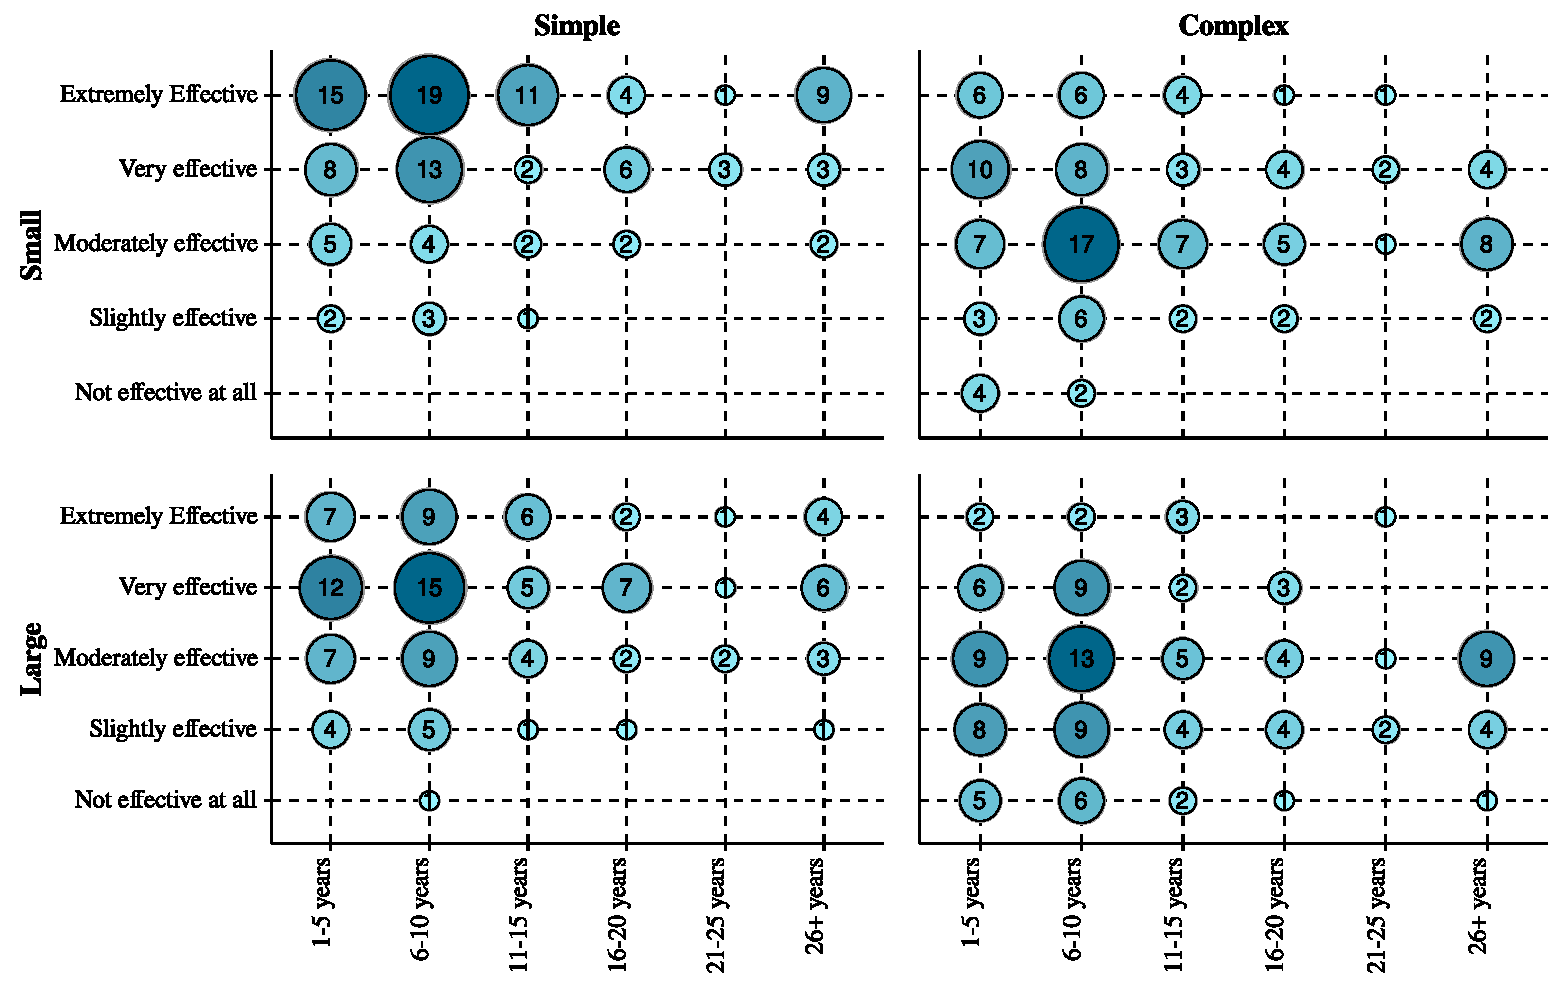
\includegraphics[width=\textwidth]{ConflictComplexityVsSize.pdf}
\caption{Effectiveness of developer tools in supporting varying levels of size and complexity (by developer experience).}
\label{size_vs_complexity}
\end{figure*}

\subsubsection{Archeology}
Archeology is an important step for many software developers, as illustrated in the following quote from P8:
\begin{displayquote}
\textit{I'm often dealing with code other people wrote... Nobody can review every pull request that goes in. So now I have to go back and do some archaeology to find out what's going on. Code is much easier to write than read.}
\end{displayquote}
P2 explains that projects make it a priority to keep a well-curated Git history because
\begin{displayquote}
\textit{That's a tool to reason about the project... if it's messy with a bunch of reverts... it's harder to figure out what was going on.	}
\end{displayquote}

\todo{add P1 quote}

However, when asked to rate the impact of \textit{Tool support for examining development history} on merge conflict resolution difficulty, developers rated it at a mean of 3.03 (A moderate amount). This places it as the least impactful of the 10 factors measured. However, P2 and P8 are both developers on open-source projects, which led us to investigate the effect of project type on history exploration's mean value. We found that open-source developers (mean of 3.60) found this to be their 3rd most impactful factor of difficulty, while closed-source developers (mean of 2.86) perceived it as the least-impactful factor. This suggests that history exploration in open source projects is a more difficult task or that tools are better at supporting the history exploration use cases that exist in closed-source development workflows.

